\section{Challenges for imaging MeerKAT data} \label{meerkat}
New interferometers like MeerKAT put additional challenges on the image reconstruction problem. First, the new instrument produce a new magnitude of data, forcing reconstruction algorithms to be highly scalable and distributable. Second, the more sensitive instruments with large field of view amplify effects which were negligible in older instruments, like non-coplanar baselines or the ionosphere.

In this work, the effects of non-coplanar baselines gets handled in more detail. The effect has a neat mathematical notation, it adds a third fourier component to the measurement equation, but breaks the two dimensional fourier relationship introduced in section \ref{intro:basic}. 


Self calibration Calibration gets not explicitly called, but 

Further issues that do not get handled here
\begin{itemize}
	\item (Beam Pattern, A Projection)
	\item Full polarization
	\item Wide band imaging
\end{itemize}

There are several challenger for imaging meerkat data. One problem is the new amount of data.

terabytes of measurements. Large image size 32k squared are the obvious problems to solve. Distributing the problem is not part of this work.

 In this work, it is focused on Wide field of view issue. 







\subsection{Wide Field of View Imaging and the third Fourier Component} \label{meerkat:wof}
The measurement equation of radio interferometers contains a third fourier component, the $w$ component. This leads to the following measurement equation \eqref{meerkat:ftsphere}.

\begin{equation}\label{meerkat:ftsphere}
V(u, v, w) = \int\int \frac{I(x, y)}{\sqrt{1 - x^2 - y ^2}} e^{2 \pi i [ux+vy+ w(\sqrt{1 - x^2 - y ^2} - 1)]} \: dx \: dy
\end{equation}

For small field of view observations, the term $\sqrt{1 - x^2 - y ^2} \approx 1$, and we arrive at the basic measurement equation \eqref{intro:basic}. For small field of view, the $w$ term can be ignored, and the image can be calculated with the inverse two dimensional non-uniform FFT. For wide field of view measurements, the $w$ term breaks the two dimensional Fourier relationship. The measurement equation \eqref{meerkat:ftsphere} can still be inverted, but the resulting algorithm has a quadratic runtime and is not feasible in practice.

Note that the image $I(x,y)$ of the wide field of view the measurement equation \eqref{meerkat:ftsphere} is still two dimensional, even though the Visibilities $V(u, v, w)$ have three. The relationship between Visibilities and image is neither the two, nor the three dimensional Fourier transform. The Visibilities represents an image on the celestial sphere. This means the image is naturally curved, and the $w$ component represents the distortion introduced by the curvature.

One can simply ignore the $w$ component, ignore the curvature and use the two dimensional Fourier Transform. The image then does not lie on a sphere, but on a tangent plane. At the tangent point (where $\sqrt{1 - x^2 - y ^2} \approx 1$, typically the image center in radio astronomy) the two reconstructions are identical. But the distortion gets more severe away from the tangent point. The image \ref{meerkat:2dfft} shows a tangent plane reconstruction over a large field of view, while \ref{meerkat:wcorrection} shows the same reconstruction but $w$ corrected. Close to the tangent point, the image center, the reconstructions both locate the point sources. At the image edges, the distortion gets severe enough to decorrelate the Visibilities and the point sources get 'torn' apart.

\begin{figure}[h]
	\centering
	\begin{subfigure}[b]{0.45\linewidth}
		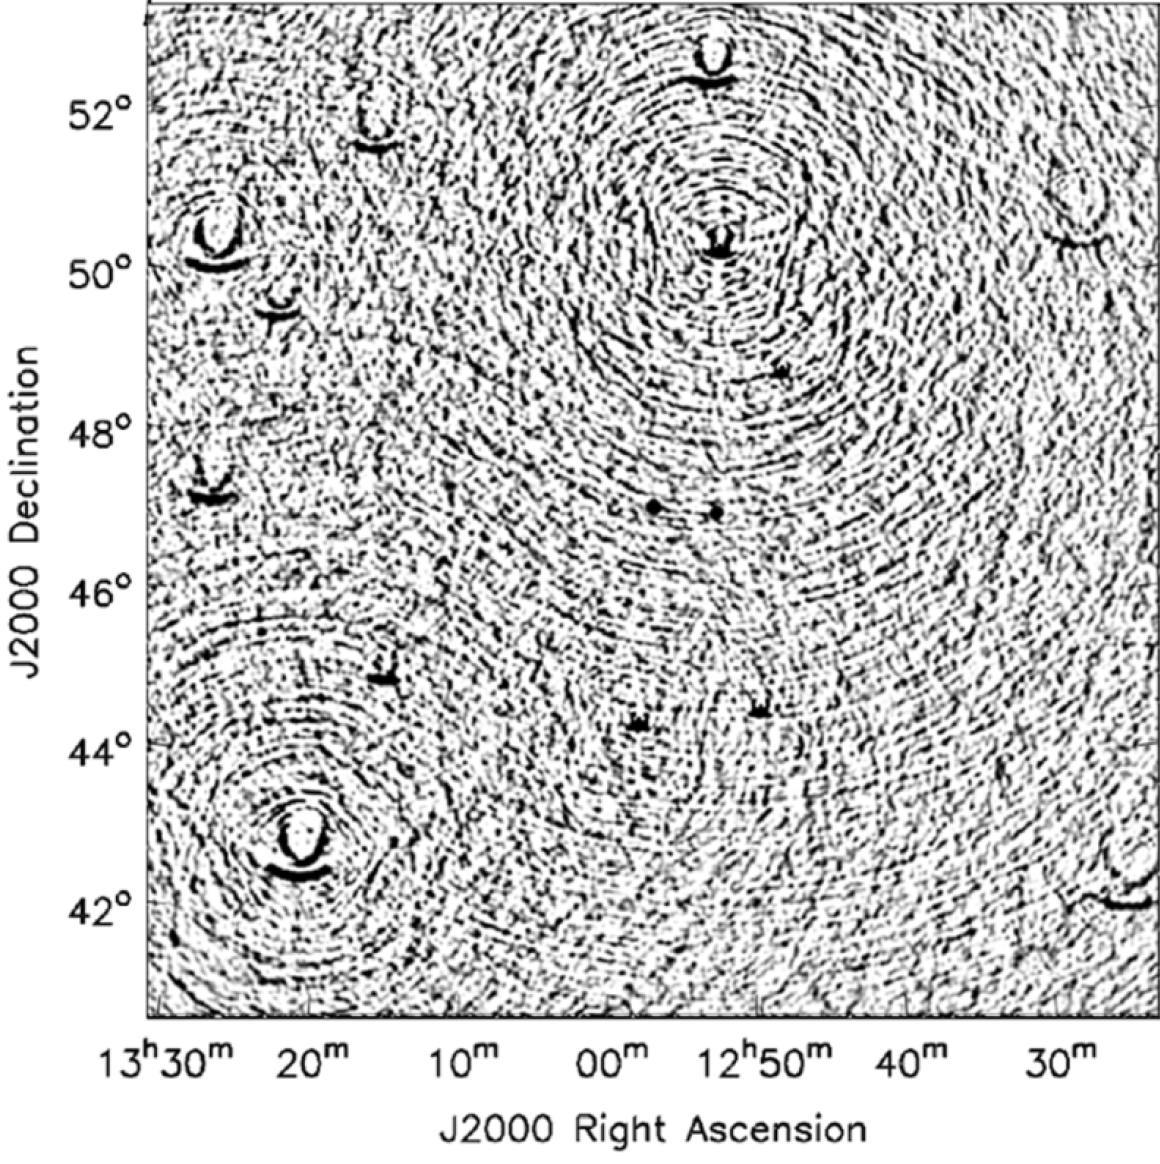
\includegraphics[width=\linewidth]{./chapters/03.challenges/w-no-correction.png}
		\caption{2D Fourier Transform.}
		\label{meerkat:2dfft}
	\end{subfigure}
	\begin{subfigure}[b]{0.45\linewidth}
		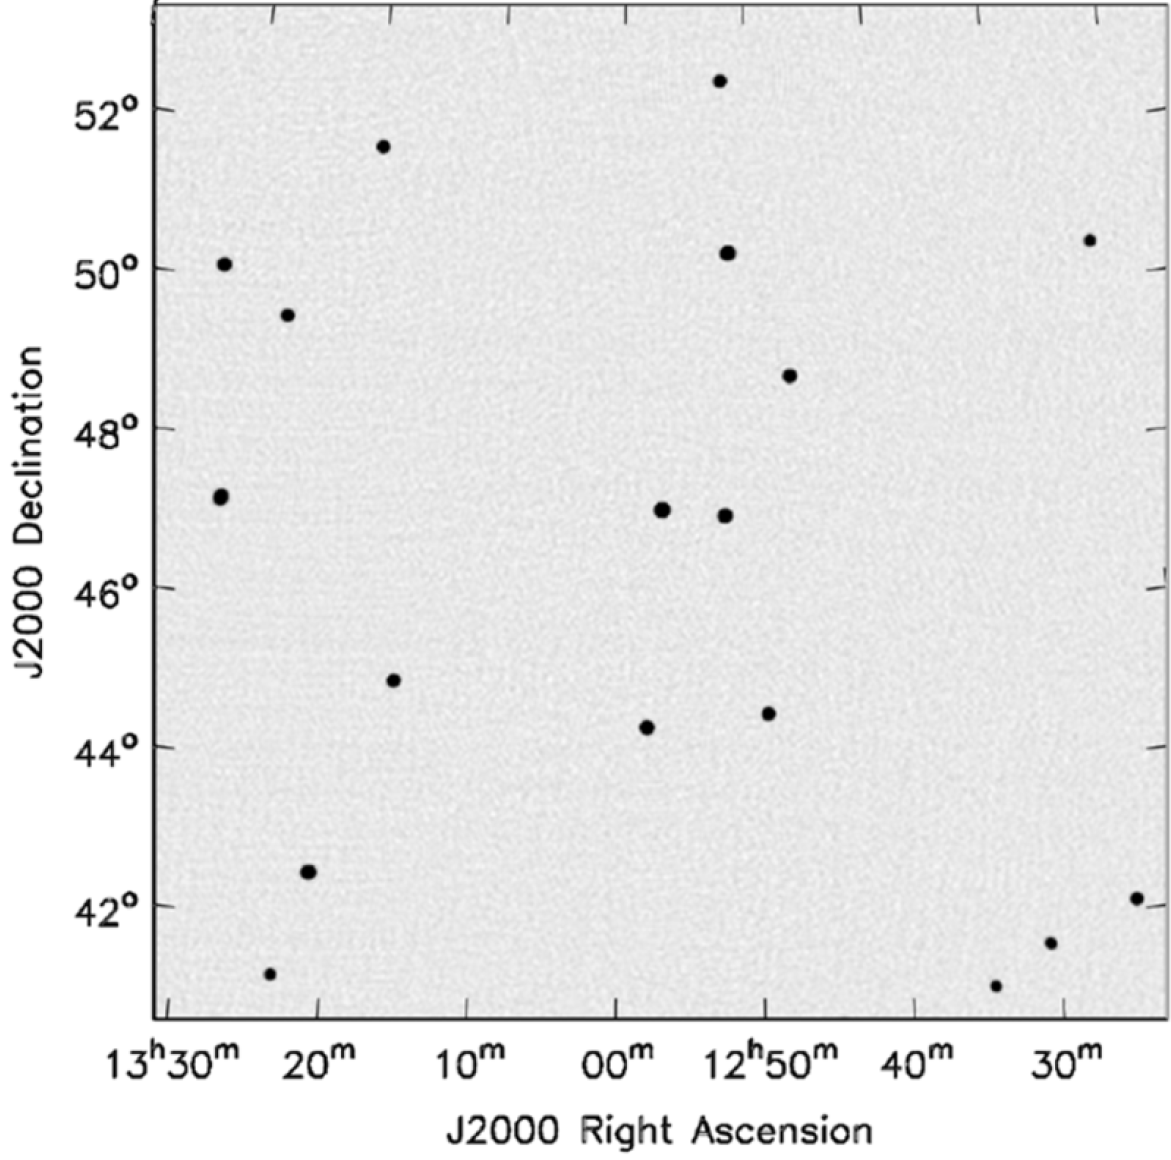
\includegraphics[width=\linewidth]{./chapters/03.challenges/w-correction.png}
		\caption{Fourier Transform with w correction.}
		\label{meerkat:wcorrection}
	\end{subfigure}
	\caption{Celestial sphere distortion on simulated data. Source: \cite{cornwell2008noncoplanar}}
	\label{meerkat:wdistortion}
\end{figure}

Image facetting

W-projection

W-stacking

So far the small Field of View inverse problem has been introduced where each antenna pair measures a Visibility of the sky brightness distribution. This leads to the small Field of View measurement equation \eqref{radio:eq:2dft}. It is identical to the two dimensional Fourier Transform. In practice the Fast Fourier Transform (FFT) is used, since it scales with $~n\:log(n)$ instead of $~n^2$ pixels.



For wide Field of View imaging, two effects break the two dimensional Fourier Transform relationship: Non-coplanar Baselines and the celestial sphere which lead to the measurement equation \eqref{radio:eq:ftSphere}. Note that for small Field of View $1 - x^2 -y ^2 \ll 1$, and \eqref{radio:eq:ftSphere} reduces to the 2d measurement equation \eqref{radio:eq:2dft}.



\subsection{Self-Calibration}
Why self calibration

Self calibration with clean




\subsection{State of the Art: WSCLEAN and the third Fourier Component} 

\cite{offringa2014wsclean} WSCLEAN

Essentially distributing the non-uniform FFT of the Major Cycle.

Architecture of W-Stacking

(talking about more recent hybrid approach, limiting the total number of ?w-stacks?)






